\begin{blocksection}
\question The \textit{Mandelbrot sequence starting at $(a, b)$} is a sequence of points in the plane recursively defined by the following: 
\begin{itemize}
    \item The first term of the sequence is $(a, b)$.
    \item If a term in the sequence is $(x, y)$, then the following term is $(x^2 - y^2 + a, 2xy + b)$.
\end{itemize}
For example, the first three terms of the Mandelbrot sequence starting at $(1, -1)$ are as follows: 
$$(1, -1)$$ 
$$(1^2 - (-1)^2 + 1, 2(1)(-1) + -1) = (1, -3)$$ 
$$(1^2 - (-3)^2 + 1, 2(1)(-3) - 1) = (-7, -7)$$
Write a higher order function \lstinline{mandelbrot_seq} that accepts two numbers, \lstinline{start_x} and \lstinline{start_y}. \lstinline{mandelbrot_seq} returns a function that takes two numbers \lstinline{x} and \lstinline{y} and returns the next term after \lstinline{(x, y)} in the Mandelbrot sequence starting at \lstinline{(start_x, start_y)}.

\begin{lstlisting}
def mandelbrot_seq(start_x, start_y):
    """ 
    >>> seq = mandelbrot_seq(1, -1)
    >>> seq(1, -1)
    (1, -3)
    >>> seq(1, -3)
    (-7, -7)
    """
    def mandelbrot_next(x, y):

        return ____________________, _______________________

    return _____________________________
\end{lstlisting}

\begin{solution}
\begin{lstlisting}
def mandelbrot_seq(start_x, start_y):
    def mandelbrot_next(x, y):
        return x ** 2 - y ** 2 + start_x, 2 * x * y + start_y
    return mandelbrot_next
\end{lstlisting}
\end{solution}

\begin{questionmeta}
    The main concept in this problem that will throw students off is that we return a tuple,
    so ensure to go over tuples if they aren't familiar with them when you walk through the doctests.
\end{questionmeta}
\end{blocksection}

\begin{blocksection}
\question Write a function \lstinline{in_or_out}, which returns \lstinline{False} if any of the first \lstinline{limit} terms of the Mandelbrot sequence starting at \lstinline{(start_x, start_y)} is a distance of more than $2$ away from the point $(0, 0)$, and \lstinline{True} otherwise. 
\begin{lstlisting}
def in_or_out(start_x, start_y, limit):
    """
    >>> in_or_out(1, -1, 1) # (1, -1) dist is sqrt(2) < 2
    True
    >>> in_or_out(1, -1, 3) # (1, -3) dist is sqrt(10) > 2
    False
    >>> in_or_out(100, 100, 0) # no terms to consider
    True
    """
    next_term = ______________________________________________
    def helper(x, y, limit):

        if ______________________________________________:
            return True

        elif ______________________________________________: 
            return False
        else: 
            next_x, next_y = next_term(x, y)

            return ___________________________________________
            
    return ______________________________________________
\end{lstlisting}
\end{blocksection}
\begin{solution}
\begin{lstlisting}
def in_or_out(start_x, start_y, limit):
    next_term = mandelbrot_seq(start_x, start_y)

    def helper(x, y, limit):
        if limit <= 0:
            return True
        elif x ** 2 + y ** 2 > 4: 
            return False
        else: 
            next_x, next_y = next_term(x, y)
            return helper(next_x, next_y, limit - 1)
            
    return helper(start_x, start_y, limit)
\end{lstlisting}
The \textit{Mandelbrot set} is the set of all points $(x, y)$ in the plane for which the Mandelbrot sequence starting at $(x, y)$ does not escape to infinity. An approximate picture of this set can be seen by plotting all the points \lstinline{(x,y)} where \lstinline{in_or_out(x, y, limit)} returns \lstinline{True} (don't worry if you don't understand this code): 
\begin{lstlisting}
for y in range(50, -50, -1):      
    for x in range(-100, 25):
        if in_or_out(x/50, y/50, 20):
            print('#', end='')
        else: 
            print(' ', end='')
    print()
\end{lstlisting}
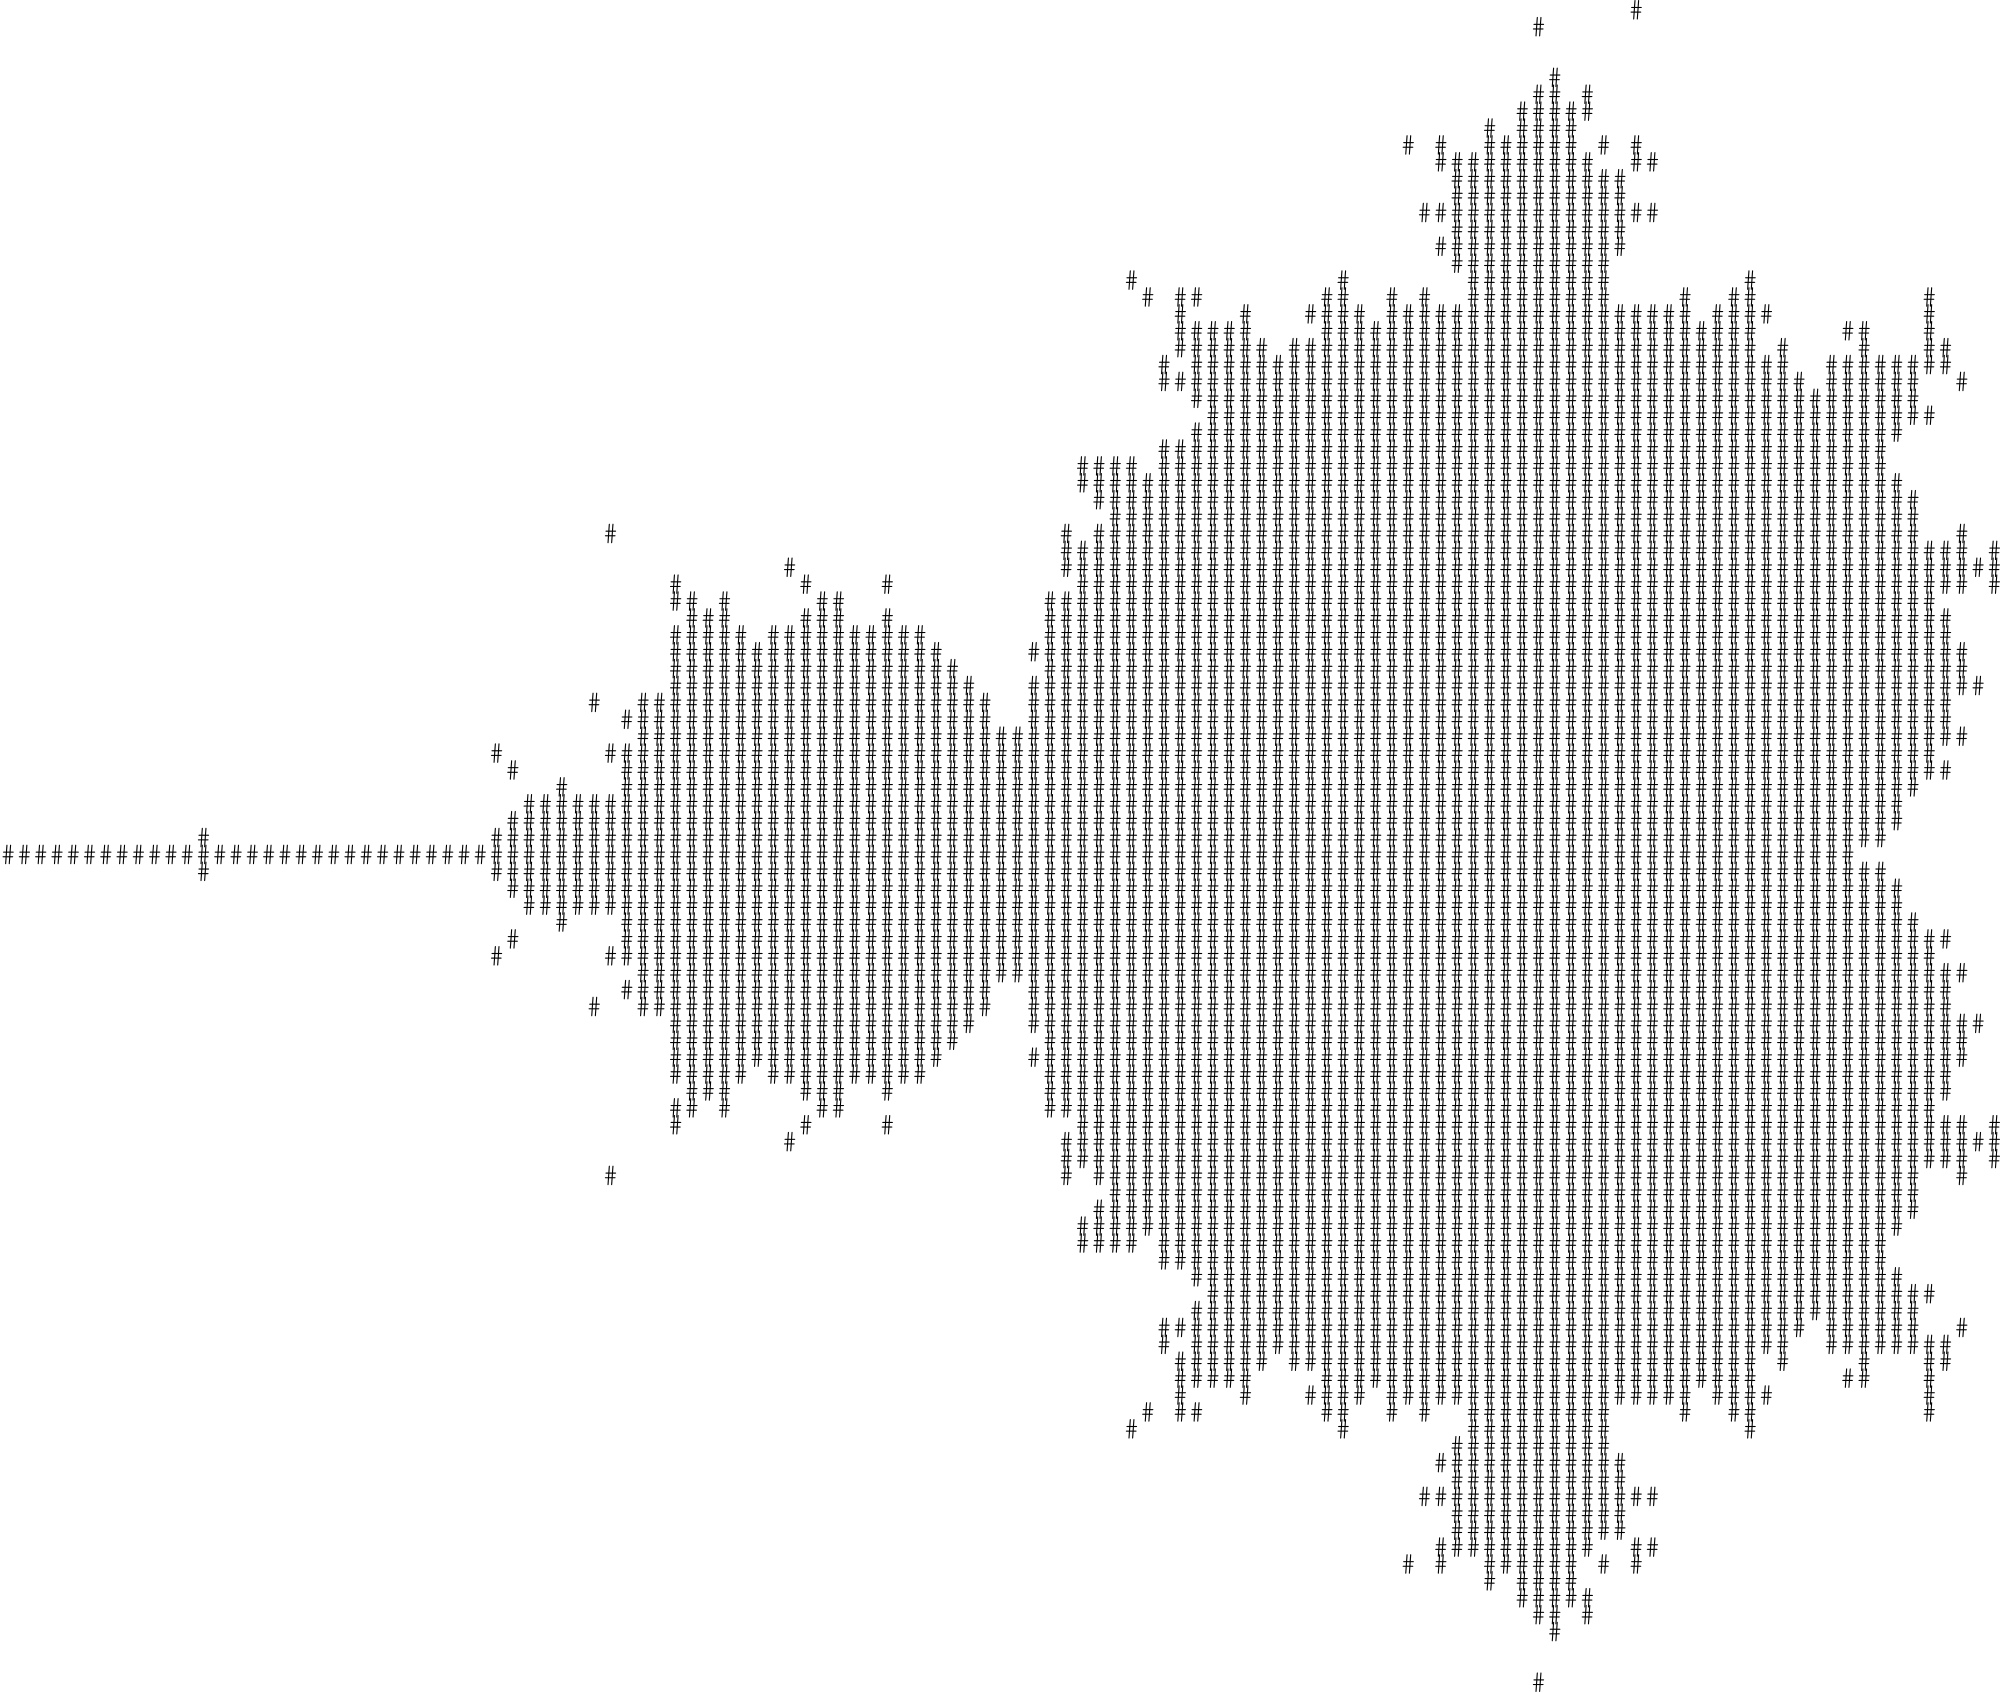
\includegraphics[width=.75\textwidth]{mandelbrot.png}
\end{solution}

\begin{questionmeta}
A major feature of this problem is that it exercises both higher order functions and recursive problem solving skills. 

Students might find the use of \lstinline{next_term} to be a little bit tricky. If this is giving your students trouble, ask them what sort of information the line \lstinline{next_x, next_y = next_term(x, y)} gives them. Hopefully, this will help them deduce that \lstinline{next_term} has to be a function that takes in two numbers and returns two numbers, and they'll make the connection with the previous part. 

The use of \lstinline{limit} as a recursive argument might be novel to some students, but it's a pretty common idea that crops up across all types of problems. I'd try to emphasize this to your students. 
\end{questionmeta}